% THIS IS AN EXAMPLE DOCUMENT FOR VLDB 2012
% based on ACM SIGPROC-SP.TEX VERSION 2.7
% Modified by  Gerald Weber <gerald@cs.auckland.ac.nz>
% Removed the requirement to include *bbl file in here. (AhmetSacan, Sep2012)
% Fixed the equation on page 3 to prevent line overflow. (AhmetSacan, Sep2012)

\documentclass{vldb}
\usepackage{graphicx}
\usepackage{balance}  % for  \balance command ON LAST PAGE  (only there!)


\begin{document}

% ****************** TITLE ****************************************

\title{Unscheduled Private Jets}

% possible, but not really needed or used for PVLDB:
%\subtitle{[Extended Abstract]
%\titlenote{A full version of this paper is available as\textit{Author's Guide to Preparing ACM SIG Proceedings Using \LaTeX$2_\epsilon$\ and BibTeX} at \texttt{www.acm.org/eaddress.htm}}}

% ****************** AUTHORS **************************************

% You need the command \numberofauthors to handle the 'placement
% and alignment' of the authors beneath the title.
%
% For aesthetic reasons, we recommend 'three authors at a time'
% i.e. three 'name/affiliation blocks' be placed beneath the title.
%
% NOTE: You are NOT restricted in how many 'rows' of
% "name/affiliations" may appear. We just ask that you restrict
% the number of 'columns' to three.
%
% Because of the available 'opening page real-estate'
% we ask you to refrain from putting more than six authors
% (two rows with three columns) beneath the article title.
% More than six makes the first-page appear very cluttered indeed.
%
% Use the \alignauthor commands to handle the names
% and affiliations for an 'aesthetic maximum' of six authors.
% Add names, affiliations, addresses for
% the seventh etc. author(s) as the argument for the
% \additionalauthors command.
% These 'additional authors' will be output/set for you
% without further effort on your part as the last section in
% the body of your article BEFORE References or any Appendices.

\numberofauthors{2} %  in this sample file, there are a *total*
% of EIGHT authors. SIX appear on the 'first-page' (for formatting
% reasons) and the remaining two appear in the \additionalauthors section.

\author{
% You can go ahead and credit any number of authors here,
% e.g. one 'row of three' or two rows (consisting of one row of three
% and a second row of one, two or three).
%
% The command \alignauthor (no curly braces needed) should
% precede each author name, affiliation/snail-mail address and
% e-mail address. Additionally, tag each line of
% affiliation/address with \affaddr, and tag the
% e-mail address with \email.
%
% 1st. author
\alignauthor
Enrique Tejera Gonzalez\\
       \affaddr{Vrije Universiteit Amsterdam}\\
       \affaddr{Amsterdam, Netherlands}\\
       \email{e.tejeragonzalez@student.vu.nl}
% 2nd. author
\alignauthor
Pawel Ulita\\
       \affaddr{Vrije Universiteit Amsterdam}\\
       \affaddr{Amsterdam, Netherlands}\\
       \email{p.k.ulita@student.vu.nl}
}
% There's nothing stopping you putting the seventh, eighth, etc.
% author on the opening page (as the 'third row') but we ask,
% for aesthetic reasons that you place these 'additional authors'
% in the \additional authors block, viz.
%\additionalauthors{Additional authors: John Smith (The Th{\o}rv\"{a}ld Group, {\texttt{jsmith@affiliation.org}}), Julius P.~Kumquat
%(The \raggedright{Kumquat} Consortium, {\small \texttt{jpkumquat@consortium.net}}), and Ahmet Sacan (Drexel University, {\small \texttt{ahmetdevel@gmail.com}})}
%\date{30 July 1999}
% Just remember to make sure that the TOTAL number of authors
% is the number that will appear on the first page PLUS the
% number that will appear in the \additionalauthors section.


\maketitle

\begin{abstract}
In this assignment we classify and visualize private jet flight patterns, 
for making it possible we have been provided with a dataset 
that contains all required information about all flights
 registered in a week of september 2016.

First of all we have to identify which flights are private jets from our dataset, 
then having created our own dataset of only private jets, we can look for usual airports and routes. 
After that we will compare locations of airports that are closed to prison 
to identify which ones are actually “rendition flights”.
\end{abstract}



\section{Introduction}
First we started with a provided dataset from September 2015, 
consisted of 200 GB of compressed ADS-B messages. 
We decoded the messages to be able to work with them 
and we extracted a sample to make the first steps of the filters 
and the code created for filtering the information that we wanted to extract from the dataset.

Another dataset of 600 GB was provided, this time information was from september of 2016.

\section{Related work}
In 2010 Matei Zaharia, Mosharaf Chowdhury, Michael J. Franklin, 
Scott Shenker, Ion Stoica from University of California, 
Berkeley proposed a new model for cluster computing called Spark. 
This system was supposed to replace the standard in 2010 which 
was MapReduce. The authors claim that a system with a wider range 
of possible programming styles than MapReduce allows is necessary. 
The two main types are: iterative jobs and interactive analytics.

The entry point of Spark applications is so called driver program. 
This application controls all of the operations on the data which then 
are issued to the cluster. The data itself is represented as RDDs, 
resilient distributed datasets. It’s a lazy and read-only representation 
of a dataset. Thanks to it the user doesn’t have to worry about parallelization and resilience.

A RDD can be created from several sources, most notably: 
a file from a shared file system (e.g. HDFS), by parallelizing a 
Scala collection, by transforming an existing RDD, by changing 
the persistence of an existing RDD. There is a collection of parallel 
operations supported by Spark. It includes reduce, collect (which 
sends the RDD back to the driver program) and foreach which allows 
invoking a function to get side effects.

The operations mentioned in the previous paragraph clearly belong to 
the functional paradigm. However, Spark allows also more imperative way 
of writing applications. This is done by using shared variables: broadcast 
variables and accumulators. The former can be used to distribute a big 
read-only piece of data to the workers. This is an optimization which prevents 
sending this structure every time an operation relying on it is performed. 
The latter can be used as a counter of any type.

Implementing RDDs was the central part of the implementation. 
RDDs are implemented as a list of objects capturing the actions which 
are supposed to be invoked on the dataset. Each RDD implements an 
interface which consists of 3 methods: getPartitions(), getIterator(partition) 
and getPreferredLocations(partition). getPartitions() returns list of partition 
IDs which contain the data. getIterator() returns an iterator used to iterating 
over a partition. getPreferredLocation() is used to achieve data locality.

\section{Technologies}
The main technology used in this assignment is Apache Spark 1.6.1 with Scala 2.10. 
Besides that we used Python 2.7. Spark was used to first filter and then analyze the dataset. 
Python was used to convert the output data from Spark to the format suitable for our visualisation.

We chose those technologies, because of several reasons. 
Apache Spark is becoming increasingly popular and is the de facto standard for big data. 
It is very modern and, provides very easy and intuitive interface. 
Besides that none of us had any practical experience with neither Spark nor Scala. 
Python is very easy to use when it comes to scripting.

\section{Managing dataset}
\subsection{Data Format}
The original dataset consists of several Apache Avro files. 
According to the schema equipped with those files they contain the following fields: sensorType, sensorLatitude, 
sensorLongitude, sensorAltitude, timeAtServer, timeAtSensor, timestamp, rawMessage, sensorSerialNumber, RSSIPacket, 
RSSIPreamble, SNR, confidence. Only sensorType, timeAtSensor, rawMessage, sensorSerialNumber are bound to be in every message.

\subsection{Preliminary data filtering}
The original dataset contains a lot of unnecessary data with each of the messages,
 i.e. only “rawMessage” and “timeAtSensor” are of importance to us. 
Filtering out the other fields lets us make the data smaller by as much as 75%.

\subsection{ADS-B Messages}
The field rawMessage contains the message received by the sensor. 
Those messages are 112 bits long. Bits 1 to 5 are called 'downlink format', 
6 to 8 'Message Subtype', 9 to 32 'ICAO Aircraft Address', 33 to 88 'Data Frame' and 89 to 112 'Parity Check'. 

In this assignment of particular importance are messages which downlink format is set to 17 (decimal) and 
the first 5 bits of 'data frame' (which are called 'Type Code') are set to some value between 1 and 4, between 9 and 18 or between 20 and 22.

'Type Code' set to values between 1 and 4 means that this is an 
identification message which contains the callsign. 
Values between 9 and 18 or between 20 and 22 indicate that this is a position message. 
Only those two types of messages are of interest to us from the context of this assignment.

For handling those messages we use a Java library provided 
by The OpenSky Network \footnote{https://github.com/openskynetwork/java-adsb}. 
It has a decoder which can decode single messages. We use it to check the type and, 
if it’s an identification message, get the callsign. 
The library has also a position decoder which can be fed 
with position messages and return a position for each of them (if possible).

\subsection{Finding suitable planes}
The major filtering part of the messages is based on callsigns. 
As our main goal is to find unscheduled private jets, it’s probably 
the best to first filter out all of the planes which don’t belong to any airlines. 
We do it by finding all of the identification messages from planes 
with either a callsign which doesn’t belong to a known airline or no callsign at all. 
From those messages we take all of the distinct ICAO24s and filter the position messages based on that.

\subsection{Decoding position messages}
Decoding position messages is not trivial in general. Each of those messages is either even or odd. 
To be able to decode a position we have to have a pair of even and odd messages which were sent near each other. 
To achieve this we have to sort the messages by the time when they were received. 
After that we use a position decoder from The OpenSky Network’s library and feed it with those messages.

Real life data is not perfect and even after sorting the messages by time rather often there are 
situations where there are multiple odd or even messages in a row. Fortunately, 
the position decoder handles incorrect situations like this one very well.

\section{Visualisation}

\subsection{Map representation}
For visualizing the extracted information we obtained maps from different sources. 
First we started using the maps from Natural Earth, provided in ESRI Shapefile format.
An ESRI shapefile consists of a main file, an index file, and a dBASE table.  The main
file is a direct access, variable-record-length file in which each record describes a shape
with a list of its vertices.  In the index file, each record contains the offset of the
corresponding main file record from the beginning of the main file.  The dBASE table
contains feature attributes with one record per feature.  The one-to-one relationship
between geometry and attributes is based on record number.  Attribute records in the
dBASE file must be in the same order as records in the main file.
Also we found another Shapefile 
which contains most of the locations of the principal airports in the World. We created a 
composition using shapefiles as layers in QGIS \footnote{QGIS is a user friendly Open Source 
Geographic Information System (GIS) licensed under the GNU General Public License}. 
With this program we were able to visualize in a 
world map all airport locations using a real scale.

All the information about countries and airports included in the shapefiles were very interesting 
for our project, the possibility of accessing it anytime only accessing the map. 
The only problem was that all the routes information could not be inserted after the creation of the 
final map, leaving no option for interaction with the user after exporting the map.

\begin{figure}
\centering
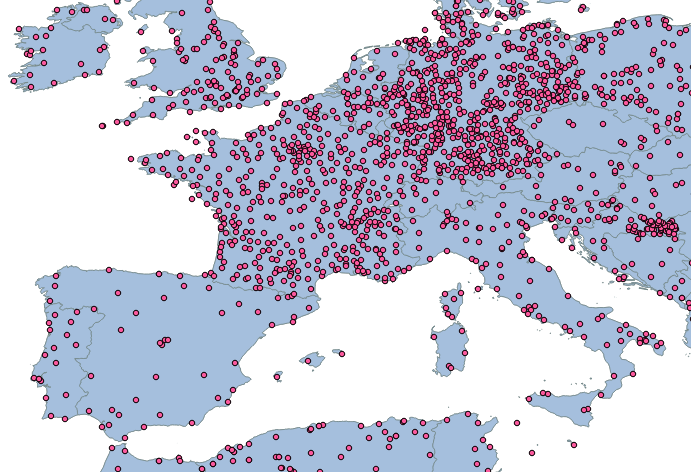
\includegraphics[width=0.47\textwidth]{Europe_mini}
\caption{Map visualisation in QGIS with layer of airports applied.}
\label{fig:Europe_mini}
\end{figure}

\subsection{Route representation}
One of the biggest problems we have when we are done with extracting 
the routes from the dataset is the fact that they are substantially more 
complex than we actually need. An obvious way to cope with this is to use 
an algorithm capable of reducing the number of points while maintaining 
a the curve shape with reasonable accuracy.

There are multiple approaches to solving this problem.
 One of them would be to remove from the line either randomly a certain 
percentage of the points or every nth point. This is a very efficient method 
in terms of computing time, but very inefficient in terms of accuracy 
and therefore should not be used for such irregular shapes as a plane route.

If the line is long enough it’s possible to remove all points besides every nth point. 
Assuming that the density is high enough this can yield acceptable results and it is 
very efficient. However, using this method will not take into account 
the shape of the line and straight parts will be overrepresented.

Another approach is known as the Ramer–Douglas–Peucker algorithm. 
It was developed by U. Ramer \cite{Ramer:polygonal}, David Douglas and Thomas Peucker \cite{Douglas:reduction}.

This algorithm focuses on removing points which have the least meaning 
in terms of the general shape. Before the algorithm starts, an arbitrary
 parameter - let’s call it d - has to be known. This parameter describes the 
accuracy of the output line. The higher it is, the less accurate the output is.

\begin{figure}
\centering
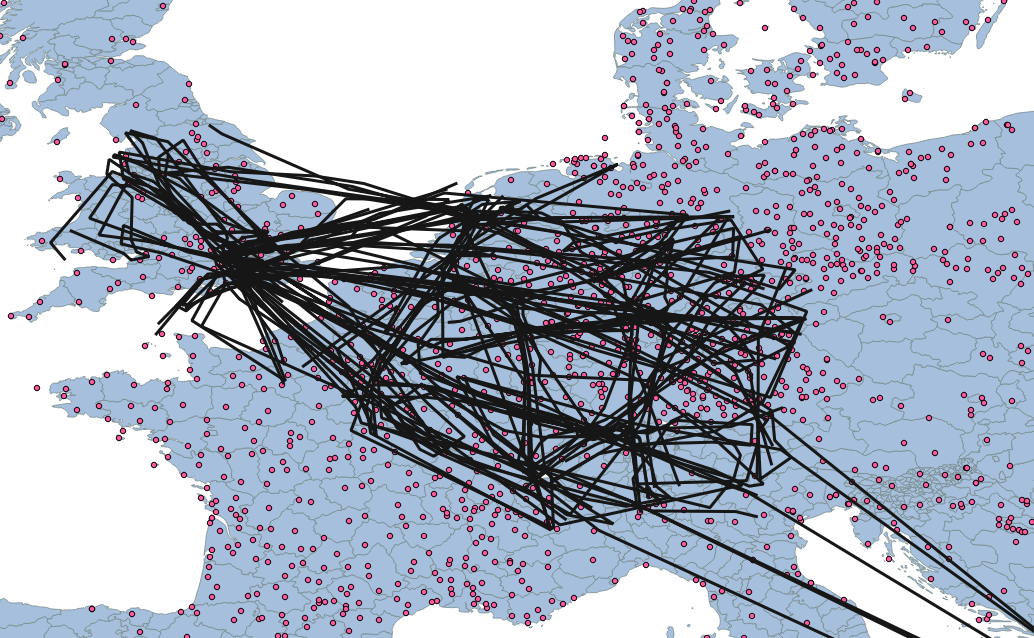
\includegraphics[width=0.47\textwidth]{europe_airports_routes_sample}
\caption{Representation of routes using first visualisation.}
\label{fig:europe_airports_routes_samplei}
\end{figure}

A simplified version of this algorithm is as follows. 
The first and the last point of the line are included in the output line. 
Let’s call them a and b, respectively. Then it is checked whether there are 
any points within the distance d from the line going through a and b. 
Those points are removed. After that the furthest point from the line is 
taken into account - let’s call it c. From now on two lines are considered: a-c and c-b. 
Those lines are then processed the in the same way. 
If no such point c exists, then the algorithm terminates.

The expected complexity of this algorithm is: \begin{displaymath}{O(n \log n)}\end{displaymath}
However, in the worst case scenario it goes up to: \begin{displaymath}{O(n^2)}\end{displaymath}

\section{Second Visualisation}
After achieving the first static visualisation we decided to make 
another one interactive, simple and intuitive, because of the aim was to 
represent flight routes we do not need so much information 
about countries and airports for printing routes. 
The best option that we found was to create a webpage, using Javascript and Json. 

\begin{figure}
\centering
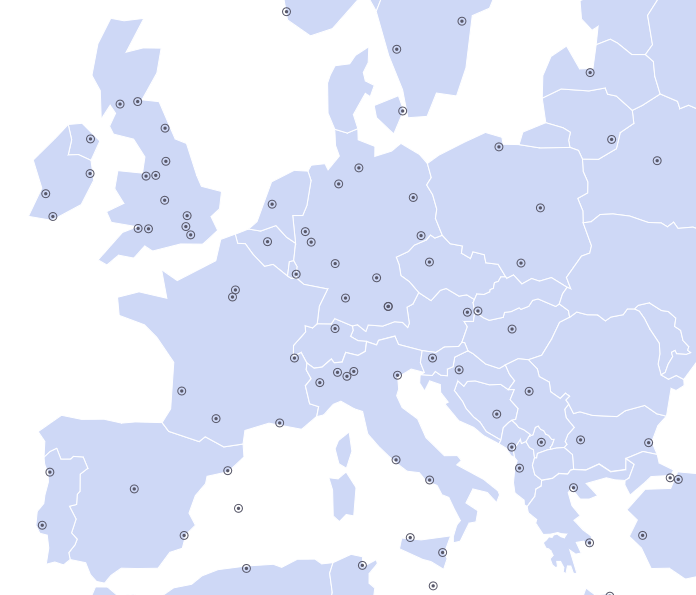
\includegraphics[width=0.47\textwidth]{js_Europe_center_few_airports}
\caption{Second visualisation using js with a few airports added.}
\label{fig:js_Europe_center_few_airportsi}
\end{figure}

This time the world map was obtained from 
Amcharts \footnote{https://www.amcharts.com/javascript-maps/}. 
They provide not only the map but diferent options for representing 
points in the map (airports in our case) and animating 
little planes through the lines created between points. 

For our project airports will be provided by the origins and 
destinations of routes extracted from the dataset, because 
for this case we cannot use airports of the World as points in the map, it could lead to confussion
because routes are made of coordinates and not all start or finish at the same position of an airport. 
Routes will be provided in the same way but instead of using shapefiles we will convert them to json files.


\section{Conclusions}
The most important part of this project was to identify 
and visualize flights which could be considered as unscheduled. 
We did that mainly by looking for planes which didn’t emit any 
callsign or their callsign didn’t belong to a known airline. 
Then those messages were grouped by ICAO24 and by date. 
Routes obtained this way were reduced using the Ramer–Douglas–Peucker algorithm. 
The planes were also annotated with information 
about the manufacturer and model. 
This approach gives us a reasonably good picture of the main routes and most popular airports. 
This is clearly visible on visualizations.

However, there are a lot of questions which we weren’t 
able to answer due to lack of time. We weren't able to extract 
unusual airports and find a reasonable heuristic for identifying 
rendition flights. We also didn’t analyze the altitudes, so we 
weren’t able to easily extract single flights within a day. 
Another problem was that we weren’t able to use the new 
dataset, because we were getting strange results. 
Due to lack of time we didn’t address those problems.
%\end{document}  % This is where a 'short' article might terminate

% ensure same length columns on last page (might need two sub-sequent latex runs)
%\balance


% The following two commands are all you need in the
% initial runs of your .tex file to
% produce the bibliography for the citations in your paper.
\bibliographystyle{abbrv}
\bibliography{LSDE_Group14_Assignment2_Report}  % vldb_sample.bib is the name of the Bibliography in this case
% You must have a proper ".bib" file
%  and remember to run:
% latex bibtex latex latex
% to resolve all references

\subsection{References}


\end{document}
